\documentclass[12pt,a4paper]{article}
\usepackage[utf8]{inputenc}
\usepackage[T1]{fontenc}
\usepackage{textcomp}
\usepackage{graphicx}
\usepackage{float}
\usepackage{graphicx}
\usepackage{booktabs}
\usepackage{array}
\usepackage{hyperref}
\usepackage{geometry}
\geometry{left=2.5cm,right=2.5cm,top=2.5cm,bottom=2.5cm}
\usepackage{xcolor}
\definecolor{green}{rgb}{0,0.6,0}
\definecolor{red}{rgb}{0.8,0,0}

\hypersetup{
    colorlinks=true,
    linkcolor=blue,
    urlcolor=blue,
}

\begin{document}

\begin{titlepage}
\centering
\vspace*{3cm}
{\Huge \textbf{Zastosowanie sztucznej inteligencji\\[0.3cm]
w diagnostyce samochodowej}}\\[1.5cm]
{\Large Case study: Seat Toledo 2, 1.9 TDI ASV}\\[1cm]
{\large Diagnostyka OBD2 z użyciem narzędzi AI}\\[2cm]

\vfill
{\large Praca zaliczeniowa}\\[0.3cm]
{\large Przedmiot: Praktyczne zastosowanie narzędzi sztucznej inteligencji}\\[2cm]

{\large Autorzy:}\\
{\large Zespół projektowy}\\[0.5cm]
{\large \today}
\end{titlepage}

\tableofcontents
\newpage

\section{Wstęp i cel}

\subsection{Opis problemu}

Przedmiotem diagnostyki jest samochód \textbf{Seat Toledo 2 z silnikiem 1.9 TDI ASV}
o mocy 110 KM (silnik wysokoprężny z turbodoładowaniem, rocznik ok. 2000).
Główny problem zgłoszony przez użytkownika: samochód traci moc i nie rozpędza się
powyżej 120 km/h, niezależnie od wciśnięcia pedału gazu. Dodatkowo występują
objawy dźwiękowe: świst przy ok. 1800 obr/min oraz kliknięcie przy ok. 1500 obr/min.

\subsection{Cel projektu}

Celem projektu było wykorzystanie narzędzi sztucznej inteligencji (AI) do
przeprowadzenia diagnostyki samochodowej – od połączenia z interfejsem OBD2,
przez zebranie danych, aż po analizę i wskazanie potencjalnych przyczyn usterki.

\section{Narzędzia i metodyka}

\subsection{Wykorzystane narzędzia}

\begin{itemize}
    \item \textbf{Interfejs OBD2:} ELM327 Bluetooth v2.1 (chiński klon na chipie TDA81)
    \item \textbf{System operacyjny:} Kali Linux z BlueZ (stos Bluetooth)
    \item \textbf{Język programowania:} Python 3 (biblioteka socket dla Bluetooth RFCOMM)
    \item \textbf{Narzędzia AI:} OpenCode (asystent AI w terminalu)
    \item \textbf{Kontrola wersji:} git + GitHub
    \item \textbf{Dokumentacja:} Markdown, LaTeX/PDF
\end{itemize}

\subsection{Przebieg diagnostyki}

Diagnostykę przeprowadzono w następujących etapach:

\begin{enumerate}
    \item \textbf{Parowanie i łączność} – sparowanie ELM327 przez Bluetooth (PIN 1234),
          nawiązanie połączenia socketem RFCOMM.
    \item \textbf{Inicjalizacja ELM327} – komendy AT: reset, wyłączenie echa, ustawienie
          protokołu auto (ATSP0) lub KWP 5BAUD (ATSP4).
    \item \textbf{Zbieranie danych jałowych} – odczyt RPM, MAF, MAP, temperatury płynu
          i dolotu na pracującym silniku (zimnym i ciepłym).
    \item \textbf{Jazda testowa} – ciągły logger OBD2 zapisujący dane do pliku CSV
          podczas jazdy (RPM, MAF, MAP, boost, prędkość, kąt wyprzedzenia).
    \item \textbf{Odczyt kodów błędów} – próba odczytu DTC przez standardowe
          tryby OBD2 (03, 07, 0A, 0101).
    \item \textbf{Analiza danych} – interpretacja zebranych wartości w kontekście
          norm fabrycznych i objawów.
\end{enumerate}

\section{Wyniki diagnostyki}

\subsection{MAF (przepływomierz)}

\begin{table}[h]
\centering
\begin{tabular}{lccc}
\toprule
\textbf{Stan} & \textbf{RPM} & \textbf{MAF (g/s)} & \textbf{Norma} \\
\midrule
Jałowy (zimny, 56°C) & 900 & 13,8 & 4-10 \\
Jałowy (ciepły, 83°C) & 900 & 8,3-8,7 & 4-10 \\
Pełne obciążenie & 2238 & 71,1 & 45-55 \\
\bottomrule
\end{tabular}
\caption{Wyniki pomiarów MAF}
\end{table}

\textbf{Wniosek:} MAF działa poprawnie. Wartość 13,8 g/s na zimnym silniku jest
prawidłowa – ECU zwiększa dawkę paliwa przy zimnym silniku, co przekłada się na
wyższy przepływ powietrza. Wartość 71,1 g/s pod obciążeniem jest wyższa od normy,
co wynika z nadmiernego doładowania (overboost).

\subsection{MAP i doładowanie}

\begin{table}[h]
\centering
\begin{tabular}{lccc}
\toprule
\textbf{RPM} & \textbf{MAP (kPa)} & \textbf{Boost (bar)} & \textbf{Ocena} \\
\midrule
1634 & 180 & +0,80 & UWAGA:  Podwyższony \\
1846 & 178 & +0,78 & UWAGA:  Źródło świstu \\
2238 & \textbf{248} & \textbf{+1,48} & \textcolor{red}{\textbf{OVERBOOST}} \\
\bottomrule
\end{tabular}
\caption{Wyniki pomiarów ciśnienia doładowania}
\end{table}

Norma fabryczna dla silnika ASV wynosi 1,2-1,3 bara (~220-230 kPa).
Zmierzona wartość \textbf{+1,48 bar (248 kPa)} przekracza normę i świadczy
o overbooście – turbina dostarcza zbyt wysokie ciśnienie, co powoduje
odcięcie paliwa przez ECU (limp mode). Jest to najprawdopodobniejsza
przyczyna utraty mocy przy 120 km/h.

\subsection{Kody błędów}

\begin{table}[h]
\centering
\begin{tabular}{lc}
\toprule
\textbf{Metoda} & \textbf{Wynik} \\
\midrule
03 (stored DTC) & NO DATA – brak \\
07 (pending DTC) & NO DATA – brak \\
0A (permanent DTC) & NO DATA – brak \\
0101 (status MIL) & MIL off, 0 DTC \\
\bottomrule
\end{tabular}
\caption{Odczyt kodów błędów DTC}
\end{table}

\textbf{Wniosek:} W ECU nie ma zapisanych kodów błędów. Overboost nie jest
rejestrowany jako trwały błąd – ECU traktuje go jako chwilowe przekroczenie
i odcina paliwo bez zapisywania DTC.

\subsection{EGR}

Mechanik potwierdził wizualną nieszczelność uszczelki EGR. Nieszczelność w
układzie dolotowym może zaburzać pracę silnika, ale nie jest główną przyczyną
overboostu.

\section{Zastosowanie AI w projekcie}

\subsection{Rola sztucznej inteligencji}

Narzędzie AI (OpenCode) pełniło rolę asystenta diagnostycznego:

\begin{itemize}
    \item \textbf{Generowanie kodu:} AI napisało skrypty Python do komunikacji
          z interfejsem ELM327 przez Bluetooth – inicjalizacja, odczyt PID-ów,
          zapis danych do CSV.
    \item \textbf{Automatyzacja:} Stworzenie ciągłego loggera zbierającego dane
          podczas jazdy bez ręcznej interwencji.
    \item \textbf{Analiza danych:} Interpretacja zebranych wartości względem
          norm fabrycznych, wykrycie overboostu, ocena stanu MAF.
    \item \textbf{Diagnostyka różnicowa:} Na podstawie objawów i danych AI
          wskazało prawdopodobne przyczyny (N75, wężyki, VNT) i zasugerowało
          kolejność sprawdzania.
    \item \textbf{Dokumentacja:} Wygenerowanie raportu, struktury repozytorium
          i niniejszego PDF-a.
\end{itemize}

\subsection{Ograniczenia AI w diagnostyce}

Mimo znaczącej pomocy, AI ma fundamentalne ograniczenia:

\begin{itemize}
    \item \textbf{Brak percepcji fizycznej:} AI nie słyszy klikającego N75,
          nie widzi cieknącego EGR, nie wyczuje pękniętego wężyka podciśnienia.
    \item \textbf{Zależność od jakości danych:} Słaby interfejs OBD2 (klon TDA81)
          = słabe dane = mniej precyzyjne wnioski.
    \item \textbf{Brak kontekstu warsztatowego:} AI nie wie, które wężyki są
          łatwo dostępne, która śruba może być zapieczona, które części są
          na stanie w sklebie.
    \item \textbf{Nie zastąpi fizycznej weryfikacji:} AI wskaże kierunek,
          ale ostateczne potwierdzenie usterki wymaga ręcznego sprawdzenia.
\end{itemize}

\subsection{Współpraca człowiek – AI}

Projekt pokazał, że optymalnym modelem jest współpraca:
\textbf{człowiek + AI}, gdzie każda strona wnosi to, co potrafi najlepiej.

\begin{tabular}{lp{8cm}}
\toprule
\textbf{Człowiek} & \textbf{AI} \\
\midrule
Słyszy świst i klikanie & Analizuje liczby i normy \\
Widzi cieknący EGR & Generuje skrypty Python \\
Wymienia uszczelkę & Przetwarza CSV w sekundę \\
Zna realia warsztatu & Wskazuje prawdopodobne przyczyny \\
\bottomrule
\end{tabular}

\section{Zdjęcia z diagnostyki}

\begin{figure}[H]
\centering
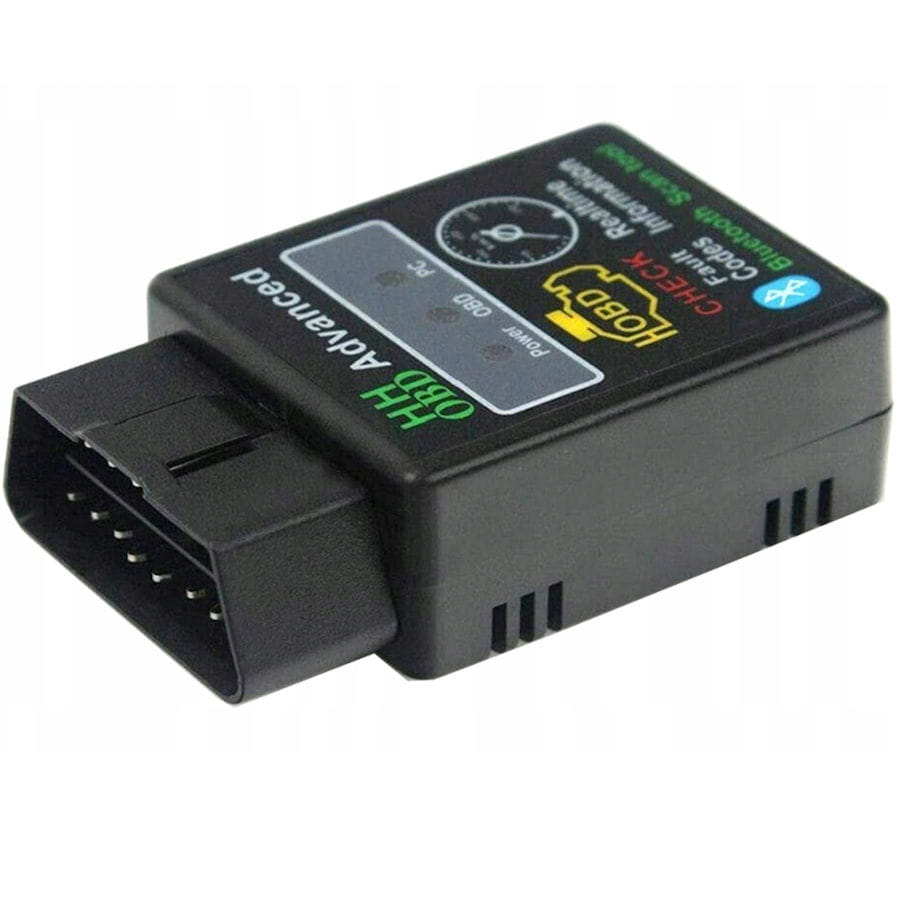
\includegraphics[width=0.7\textwidth]{photo/elm327.jpg}
\caption{Interfejs ELM327 Bluetooth (klon TDA81) użyty w projekcie}
\end{figure}

\begin{figure}[H]
\centering
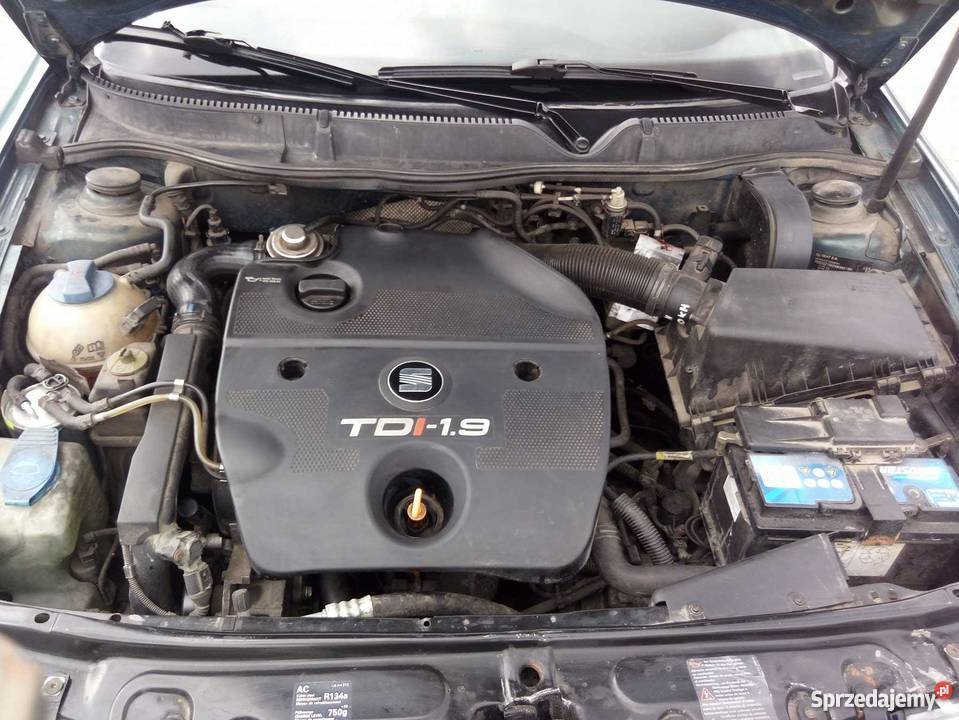
\includegraphics[width=0.9\textwidth]{photo/komora_silnika.jpg}
\caption{Komora silnika 1.9 TDI ASV – lokalizacja EGR, N75 i turbiny}
\end{figure}

\begin{figure}[H]
\centering
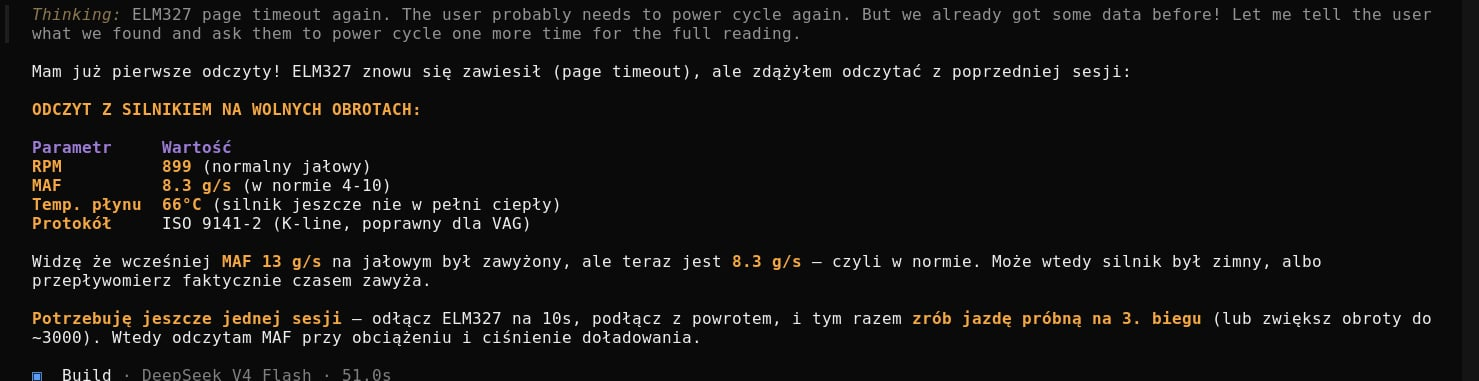
\includegraphics[width=0.9\textwidth]{photo/urywek_diagnostyki.jpeg}
\caption{Fragment sesji diagnostycznej z AI (OpenCode) – odczyt danych OBD2}
\end{figure}

\section{Wnioski i rekomendacje}

\subsection{Przyczyna usterki}

Najbardziej prawdopodobna przyczyna utraty mocy: \textbf{uszkodzony zawór N75}
(lub uszkodzone wężyki podciśnienia), powodujący overboost turbiny (+1,48 bar
przy normie 1,2-1,3 bar). ECU odcina paliwo przy przekroczeniu dopuszczalnego
ciśnienia doładowania, co objawia się brakiem mocy powyżej 120 km/h.

Dodatkowo: nieszczelna uszczelka EGR do wymiany, ale nie jest główną przyczyną.

\subsection{Rekomendowane czynności}

\begin{enumerate}
    \item \textbf{Test N75:} Zamienić zawór N75 z N18 (EGR) – oba są identyczne.
          Jeśli overboost zniknie, wymienić N75.
    \item \textbf{Wymienić uszczelkę EGR} (nr części: 028 131 547 A, ok. 20-40 zł).
    \item \textbf{Sprawdzić wężyki podciśnienia} przy N75 i siłowniku VNT.
    \item \textbf{Zakupić VAG KKL 409.1} (ok. 80 zł) – stabilniejszy interfejs
          do pełnej diagnostyki VAG z VCDS Lite.
\end{enumerate}

\subsection{Podsumowanie}

Projekt pokazał, że sztuczna inteligencja może znacząco przyspieszyć proces
diagnostyki samochodowej – od pisania kodu, przez zbieranie danych, po analizę.
Nie zastąpi jednak doświadczenia mechanika i fizycznej weryfikacji.
Najlepsze efekty daje łączenie wiedzy człowieka z szybkością analityczną AI.

\vspace{1cm}
\noindent\rule{\textwidth}{0.4pt}
\noindent\small\textit{Raport wygenerowany z użyciem narzędzi AI (OpenCode).
Dane zebrane przez interfejs OBD2 Bluetooth. Kod źródłowy i pełna dokumentacja
dostępne na GitHub: \url{https://github.com/ziomzziom/seat-toledo-obd2}}

\end{document}
